%% Based on a TeXnicCenter-Template by Preetham Aghalaya Manjunatha.
%%%%%%%%%%%%%%%%%%%%%%%%%%%%%%%%%%%%%%%%%%%%%%%%%%%%%%%%%%%%%

%------------------------------------------------------------
%
\documentclass[letterpaper,12pt, onecolumn]{article}%
%Options -- Point size:  10pt (default), 11pt, 12pt
%        -- Paper size:  letterpaper (default), a4paper, a5paper, b5paper
%                        legalpaper, executivepaper
%        -- Orientation  (portrait is the default)
%                        landscape
%        -- Print size:  oneside (default), twoside
%        -- Quality      final(default), draft
%        -- Title page   notitlepage, titlepage(default)
%        -- Columns      onecolumn(default), twocolumn
%        -- Equation numbering (equation numbers on the right is the default)
%                        leqno
%        -- Displayed equations (centered is the default)
%                        fleqn (equations start at the same distance from the right side)
%        -- Open bibliography style (closed is the default)
%                        openbib
% For instance the command
%           \documentclass[a4paper,12pt,leqno]{article}
% ensures that the paper size is a4, the fonts are typeset at the size 12p
% and the equation numbers are on the left side

\usepackage{amssymb,amsmath} %[fleqn] left alignment of equations
\usepackage{amsfonts}
\usepackage{mathabx}
\usepackage{mathtools}
\usepackage{mathrsfs}
%\usepackage{amssymb}%
\usepackage{graphics}
\usepackage{graphicx}
\usepackage[]{afterpage}
\usepackage{setspace}
\usepackage{epsfig}
\usepackage{todonotes}
%\usepackage[titles]{tocloft}
\usepackage{calc}
\usepackage[english]{babel}
\usepackage{blindtext}
\usepackage{fancyhdr}
\usepackage{fancybox}
\usepackage[normalem]{ulem}
%\usepackage{tikz}
%\usetikzlibrary{calc,shapes}
%\usepackage[latin1]{inputenc}
%\usepackage[utf8]{inputenc}
\usepackage{inputenc}
%\usepackage{undertilde}
\usepackage{epstopdf}
\usepackage{framed}
\usepackage{pdfpages}
\usepackage{csquotes}
\usepackage{microtype}
\usepackage{cancel}
\usepackage{caption}
\usepackage[authoryear, sort]{natbib}
%\usepackage[citestyle = authoryear, bibstyle = numeric, uniquename = init, firstinits = true, sorting = nyt, maxcitenames = 2, maxbibnames = 99, backend=bibtex]{biblatex}   
%\addbibresource{Report-CrackThruRobots.bib} \renewcommand*{\nameyeardelim}{\addcomma\space}

%\usepackage{subcaption}
\usepackage{float}
\usepackage{subfig} %[lofdepth,lotdepth]
%\usepackage{subfigure}

%\usepackage{xfrac}
%\usepackage{lipsum}
%\usepackage{appendix} %[titletoc]
%\usepackage[all]{hypcap}
\usepackage{stackrel}
\usepackage{bigints}
\usepackage{tabularx}
\usepackage{array}
\usepackage{multirow}
\usepackage{enumitem}
\usepackage{longtable}
\usepackage{supertabular}
\usepackage{url}
\usepackage{parskip}
\usepackage{tikz}
\usepackage{times}	%\usepackage{PTSansNarrow}  \usepackage{courier}
\usepackage[T1]{fontenc}
\usetikzlibrary{matrix}
\usepackage{colortbl}
\usepackage{xcolor}
\usepackage{tabu}
\usepackage[nottoc,numbib]{tocbibind}
\usepackage[toc,page]{appendix}
\usepackage{chngcntr}
%\usepackage{makeidx} \makeindex 
\usepackage{mfirstuc}
\usepackage{lineno} 
%\usepackage[bottom]{footmisc}
\usepackage[top=0.75in, bottom=1in, left=1.in, right=1.in]{geometry}

\usepackage[hidelinks,breaklinks]{hyperref}
\hypersetup{
    %bookmarks=true,         % show bookmarks bar?
    unicode=false,          % non-Latin characters in Acrobat’s bookmarks
    pdftoolbar=true,        % show Acrobat’s toolbar?
    pdfmenubar=true,        % show Acrobat’s menu?
    pdffitwindow=false,     % window fit to page when opened
    pdfstartview={Fit},    % fits the width of the page to the window //FitH
    pdftitle={Image Analysis for Defect Detection in
Infrastructures},    % title
    pdfauthor={Preetham Aghalaya Manjunatha},     % author
    pdfsubject={Displacement Field},   % subject of the document
    pdfcreator={PdfLaTeX},   % creator of the document
    pdfproducer={Texmaker}, % producer of the document
    pdfkeywords={Structural Health Monitoring,} {Displacement Measurement,} {Structural Dynamics,} {Depth Sensors} % list of keywords
    pdfnewwindow=true,      % links in new window
    colorlinks=true,       % false: boxed links; true: colored links
    linkcolor =  blue,  %[rgb]{0,0.3,0.3},          % color of internal links
    citecolor= blue,        % color of links to bibliography
    filecolor=black,      % color of file links
    urlcolor=blue           % color of external links
}
\usepackage{listings}
\usepackage[]{mcode}
\usepackage[all]{hypcap}
\usepackage[nameinlink,capitalise]{cleveref} %\crefname{section}{§}{§§}
\usepackage[explicit]{titlesec}
\titlespacing\section{0pt}{10pt plus 4pt minus 2pt}{0pt plus 2pt minus 2pt}
\titlespacing\subsection{0pt}{10pt plus 4pt minus 2pt}{0pt plus 2pt minus 2pt}
\titlespacing\subsubsection{0pt}{10pt plus 4pt minus 2pt}{0pt plus 2pt minus 2pt}

%% New commands
%%--------------------------------------------------------------------
\newcommand{\HRule}{\rule{\linewidth}{0.5mm}}
%\parskip=1cm
%\setlength{\parskip}{0.2cm}
\setlength{\parindent}{0.25in}

%% Biblatex cite author hyperlinks
%\DefineBibliographyStrings{english}{%
%  references = {Bibliography},
%}

%\DeclareFieldFormat{bibentrysetcount}{\mkbibparens{\mknumalph{#1}}}
%\DeclareFieldFormat{labelnumberwidth}{\mkbibbrackets{#1}}
%%
%\defbibenvironment{bibliography}
%  {\list
%     {\printtext[labelnumberwidth]{%
%    \printfield{prefixnumber}%
%    \printfield{labelnumber}}}
%     {\setlength{\labelwidth}{\labelnumberwidth}%
%      \setlength{\leftmargin}{\labelwidth}%
%      \setlength{\labelsep}{\biblabelsep}%
%      \addtolength{\leftmargin}{\labelsep}%
%      \setlength{\itemsep}{\bibitemsep}%
%      \setlength{\parsep}{\bibparsep}}%
%      \renewcommand*{\makelabel}[1]{\hss##1}}
%  {\endlist}
%  {\item}
%
%\DeclareNameAlias{sortname}{last-first}

%\DeclareCiteCommand{\cite}
%  {\usebibmacro{prenote}}
%  {\usebibmacro{citeindex}%
%   \printtext[bibhyperref]{\usebibmacro{cite}}}
%  {\multicitedelim}
%  {\usebibmacro{postnote}}
%
%\DeclareCiteCommand*{\cite}
%  {\usebibmacro{prenote}}
%  {\usebibmacro{citeindex}%
%   \printtext[bibhyperref]{\usebibmacro{citeyear}}}
%  {\multicitedelim}
%  {\usebibmacro{postnote}}
%
%\DeclareCiteCommand{\parencite}[\mkbibparens]
%  {\usebibmacro{prenote}}
%  {\usebibmacro{citeindex}%
%    \printtext[bibhyperref]{\usebibmacro{cite}}}
%  {\multicitedelim}
%  {\usebibmacro{postnote}}
%
%\DeclareCiteCommand*{\parencite}[\mkbibparens]
%  {\usebibmacro{prenote}}
%  {\usebibmacro{citeindex}%
%    \printtext[bibhyperref]{\usebibmacro{citeyear}}}
%  {\multicitedelim}
%  {\usebibmacro{postnote}}
%
%\DeclareCiteCommand{\footcite}[\mkbibfootnote]
%  {\usebibmacro{prenote}}
%  {\usebibmacro{citeindex}%
%  \printtext[bibhyperref]{ \usebibmacro{cite}}}
%  {\multicitedelim}
%  {\usebibmacro{postnote}}
%
%\DeclareCiteCommand{\footcitetext}[\mkbibfootnotetext]
%  {\usebibmacro{prenote}}
%  {\usebibmacro{citeindex}%
%   \printtext[bibhyperref]{\usebibmacro{cite}}}
%  {\multicitedelim}
%  {\usebibmacro{postnote}}
%
%\DeclareCiteCommand{\textcite}
%  {\boolfalse{cbx:parens}}
%  {\usebibmacro{citeindex}%
%   \printtext[bibhyperref]{\usebibmacro{textcite}}}
%  {\ifbool{cbx:parens}
%     {\bibcloseparen\global\boolfalse{cbx:parens}}
%     {}%
%   \multicitedelim}
%  {\usebibmacro{textcite:postnote}}

\DeclareMathOperator{\E}{\mathbb{E}}
%% Begin document
%%--------------------------------------------------------------------
\begin{document}
    \thisfancypage{%
    \setlength{\fboxsep}{4pt}%
    \setlength{\shadowsize}{0pt}%
    \shadowbox}{}
%	\doublebox}{} 
\begin{titlepage}
\begin{center}

% Upper part of the page


\includegraphics[scale = 0.4]{./USCsealblack.pdf}\\[0.5cm]

\includegraphics[scale = 0.25]{./ming}\\[0.5cm]

\includegraphics[scale = 0.25]{./sonny}\\[0.5cm]

\textsc{\Large A Project Report on}\\[0.25cm]



% Title
\HRule \\[0.4cm]
{ \huge \bfseries Feature Extraction, Classification and Multi-class Error Analysis of Sewer Pipeline Images}\\[0.1cm]
\HRule \\[0.5cm]


% Author and supervisor
\large \underline{Under the Supervision of}\\
Professor Keith Jenkins \\ %\footnote{Email: masri@usc.edu}\\
Ming Hsieh Department of Electrical Engineering\\
University of Southern California\\
\vspace{0.3in}


\begin{minipage}{0.4\textwidth}
\begin{flushleft} \large
\emph{Author:}\\
Preetham \textsc{Aghalaya} Manjunatha \\
USC, Dept. of Civil
\end{flushleft}
\end{minipage}%
\begin{minipage}{0.4\textwidth}
\begin{flushright} \large
\emph{Author:} \\
Shravan  \textsc{Ravi} \\
USC, Dept. of Electrical
\end{flushright}
\end{minipage}


%\large \underline{Submitted By}\\
%Preetham Aghalaya Manjunatha  %\footnote{Email: aghalaya@usc.edu}
%\\USC ID: 7356627445\\
%Sonny Astani Department of Civil and Environmental Engineering\\University of Southern California\\
%and \\
%Shravan Ravi \\
%USC ID: 9241187852 \\
%Ming Hsieh Department of Electrical Engineering

\vspace{0.3in}
% Bottom of the page
\large \underline{Submitted On}\\
\large {December 08, 2014}

\end{center}
\end{titlepage}


  

\pagenumbering{roman}

% Table Of Contents
\cleardoublepage\phantomsection
\renewcommand{\contentsname}{Table of Contents}
%\pdfbookmark{\contentsname}{toc}
\tableofcontents

% Line spacing
\setstretch{1}

% List of tables
\addtocontents{lot}{\vspace*{-\baselineskip}}
\addtocontents{lot}{\protect\addvspace{0.25in}}%
\cleardoublepage\phantomsection
\listoftables

% List of figures
\addtocontents{lof}{\vspace*{-\baselineskip}}
\addtocontents{lof}{\protect\addvspace{0.25in}}%
\cleardoublepage\phantomsection
\listoffigures

\cleardoublepage\phantomsection
\section*{Abstract}
\addcontentsline{toc}{section}{Abstract}
\noindent
Object classification is an active research in the field of computer vision and image processing. In this project, a medium-scale data is manually labeled and used to train classifiers. Non-linear classifiers such as Support Vector Machine (SVM) and Feed-forward neural Networks (FFNN) are used to predict the testing set labels. The results look very promising for large-scale object recognition. Also, it was found that a large training set reduces overfitting and improves the classification accuracy. Lastly, an attempt has been made to understand the generalization bound for multiple classes. 

\clearpage
\pagenumbering{arabic}	
\setcounter{page}{1}



%--------------------------------------------- Start of main matter -----------------------------------------------
%\linenumbers
%%%%%%%%%%%%%%%%%%%%%%%%%%%%%%%%%%%%%%%%%%%%%%%%%%%%%%%%%%%%%%%%%%%%%%%%%%%%%%%%%%%%%%%%%%%%%%%%%%%%%%%%%%%%%%%%%%%%%%%%%%%%%%%
\section{Introduction}
\noindent
Fatigue and failure are common in civil infrastructures, mechanical and aerospace systems and other applications. It is important to perform condition assessment regularly in order to minimize serious structural failures. In Structural Health Monitoring (SHM), the focus is on vibration-based methods that have been practiced for more than four decades. However, due to the development of accurate, robust and inexpensive visual sensors, vision-based autonomous SHM techniques have gained more attention. Thus, visual inspection is the most commonly used technique to assess the condition of almost all infrastructure systems \citep{jahanshahi2011multi-image}.

Civil infrastructures play an important role in the development of a country`s economy. The infrastructure cost in the US alone is more than \$20 trillion \cite{iyer2013automated}. According to the American Society of Civil Engineers` (ASCE) report, there are an estimated 0.7 to 0.8 million miles of public sewer mains in the United States \cite{asce2013}. Many of these pipelines were installed after World War II and are aging down. Due to the inadequate human resources, not every section of the pipe gets the required attention. Operational and maintenance cost of these pipelines itself requires billions of dollars every year. An irregular and non-periodic trend of sewer-pipe inspection jeopardizes the structural integrity of the waste water mains, thus increasing the possibility of untreated sewage discharge into the surroundings. A novel and innovative approach to classify healthy and unhealthy water mains is required to reduce human intervention. This system can improve the decision making ability based on objectivity, rather than on a subjective human perspective. This project includes feature extraction, classification and error analysis of sewage mains.

A vast number of videos are recorded by sending an unmanned vehicle through sewer pipelines. Analyzing these videos requires experienced human inspectors and hours of laborious visual inspection. In general, visual inspection by humans are very subjective. A damaged sewer pipe can induce a threat to the ground water sources and can be responsible for environmental issues and spread of epidemics. These factors motivate the need for autonomous vision-based techniques that eliminate the subjectivity to which humans are prone with minimal human intervention. 

\subsection{Related work}
\noindent
In a Closed-Circuit-Television (CCTV)-based monitoring system, \cite{fieguths99} used digital image processing to detect the cracks in underground pipes by means of statistical parameters such as samples, mean, variance and cross-correlation with the crack pixels and their surrounding window. Although this method is able to extract features like cracks and, to some extent, joint openings of the buried pipe, it failed to minimize false positives. Again, using a warped tunnel vision by a tool called Sewer Scanner and Evaluation Technology (SSET), \cite{iseley}, \cite{Sinha200658} and \cite{iyer2013automated} exhibited a method that extracts the crack (eliminating joints, holes and laterals) from the buried pipeline images. This is done by using the statistical filters for crack detection followed by cleaning and linking operations. Similarly, \cite{iyer_shiva} worked on multiple crack detection algorithms based on contrast enhancement, morphology, non-linear filtering and curvature evaluation of crack patterns. It is shown that morphological characters such as branches, thickness, and orientation of cracks can be exploited well for their autonomous recognition. Further, with the concept of Bayesian classification, mathematical morphological processes, and segmentation by thresholding, \cite{Sinha200647} studied the feature extraction methods for multiple cracks and joints in the sewer pipeline.

All of the prior works in the field of civil engineering are limited in defect detection from color or grayscale images using edge detection, mathematical morphology or other matched filter related algorithms. Edge detection algorithms are capable of detecting sewer pipeline features, but at the same time it is practically impossible to exclude noisy pixels or edges. Mathematical morphology works well for uniform textural images, but when the image is random textured, choosing a valid structuring element is difficult. In practice, pipeline infrastructures are comprised of complex shapes, and textures and non-uniform intensity are spread around the crack regions. In addition, only a small-scale image dataset (<500) are analyzed in the published work. 

\subsection{Contribution}
\noindent
Currently, there hardly exists any public benchmark datasets for pipelines in general, that are labeled and consist of a respectable amount of images/videos. In this work, special consideration is taken in order to prepare a labeled database consisting of a few thousand images from recorded sewer-pipe videos. As the first task, hundreds of these videos have to be converted to images, followed by the preparation of a sample dataset. A sample dataset consists of training, validation and testing images. After obtaining the image dataset, a few pre-processing algorithms such as image in-painting (text removal), super-resolution and denoising are to be performed.  Image features are extracted automatically by using the bags-of-features method proposed by \cite{csurka2004visual}. Once the features are obtained, a nine-class object classification problem is solved by using two non-linear classifiers. Furthermore, inspired by the VC generalization bound for binary class problems, an attempt had been made to understand and deduce a generalization bound for multi-class problems involving support vector machines (SVM) and Feed-forward Neural Networks (FFNN).


\subsection{Scope}
\noindent
\Cref{sec:project_setup} introduces the problem formulation and setup. In \Cref{sec:methodology} the various methods involved in this work are presented. The implementation of the proposed method is discussed in \Cref{sec:implementation}. Results and interpretation are provided in \Cref{sec:final_results} and \Cref{sec:interp} respectively. Lastly, this work is concluded by summarizing the findings and suggesting a few recommendations for future work in \Cref{sec:summary_conclusion}.


%%%%%%%%%%%%%%%%%%%%%%%%%%%%%%%%%%%%%%%%%%%%%%%%%%%%%%%%%%%%%%%%%%%%%%%%%%%%%%%%%%%%%%%%%%%%%%%%%%%%%%%%%%%%%%%%%%%%%%%%%%%%%%%
\section{Project Formulation and Setup} \label{sec:project_setup}
\noindent
The proposed method deals with classifying medium-scale image datasets into multiple classes. Among the several multiclass classifiers available, few can be generalized as direct extensions of the binary clasifers. 

A classification task usually involves separating data into training and testing sets. Each instance in the training set contains one \enquote{target value} (i.e. the class labels) and several \enquote{attributes} (i.e. the features or observed variables). The goal of the learning algorithm is to produce a model (based on the training data) which predicts the target values of the test data given only the test data attributes. 

Due to the high complexity of the problem, we decided to use two robust multiclass classifiers, namely Support Vector Machines (SVMs) and Neural Networks(NN) as both these classifiers are known to perform well for large multiclass classification \citep{jahanshahi2013innovative, csurka2004visual}. Both these models have been explained briefly below. 

\subsection{Support Vector Machine (SVM)}
\noindent
Given a training datasets and its labels ($x_i, y_i$) $i=1,\ldots,l$ where $x_i \in \mathrm{R}^N$ and $y \in {-1, 1}^l$, SVMs satisfy the unconstrained optimization problem:
\begin{equation}
\begin{split}
\min\limits_{w, b, \xi} \quad & \frac{1}{2} W^T W + C \sum\limits_{i=1}^{l} \xi_i \\
\text{subject to} \quad &y_i(W^T \phi(x_i)+b) \geq 1 - \xi_i \\
&\xi_i \geq 0
\end{split}
\end{equation}
Here training vectors xi are mapped into a higher (maybe infinite) dimensional space by the function $\phi$. SVM finds a linear separating hyperplane with the maximal margin in this higher dimensional space. C > 0 is the penalty parameter of the error term. $K(x_i, x_j) ≡ \phi(x_i)^T phi(x_j)$ is called the kernel function. In this work radial basis function is used as the kernel:
\begin{equation}
K(x_i, x_j) = exp(-\gamma \left\lVert x_i - x_j \right\rVert), \gamma > 0
\end{equation}
SVM requires that each data instance is represented as a vector of real numbers. Hence, if there are categorical attributes, we first have to convert them into numeric data. Scaling before applying SVM is very important. The main advantage of scaling is to avoid attributes in greater numeric ranges dominating those in smaller numeric ranges. Another advantage is to avoid numerical difficulties during the calculation. Because kernel values usually depend on the inner products of feature vectors, e.g. the linear kernel and the polynomial kernel, large attribute values might cause numerical problems. We thus linearly scaled each attribute to the range [0 , 1]. 

In general, the RBF kernel is a reasonable first choice. This kernel nonlinearly maps samples into a higher dimensional space so it, unlike the linear kernel, can handle the case when the relation between class labels and attributes is nonlinear. Furthermore, the linear kernel is a special case of RBF. since the linear kernel with a penalty parameter C has the same performance as the RBF kernel with some parameters (C, $\gamma$). The SVM algorithms were implemented using LIBSVM is an integrated software for support vector classification, (C-SVC, nu-SVC) which supports multiclass classification. 

A pictorial representation of the flow of the algorithm used to obtain the model and classify test images is shown in \cref{fig:svmflow}. This is an implementation of an already existing approach; basically training the classifier using optimal parameters obtained through some sort of validation procedure and then testing this formed model on unseen data.
\begin{figure}[!hbtp]
 	  \centering
 	   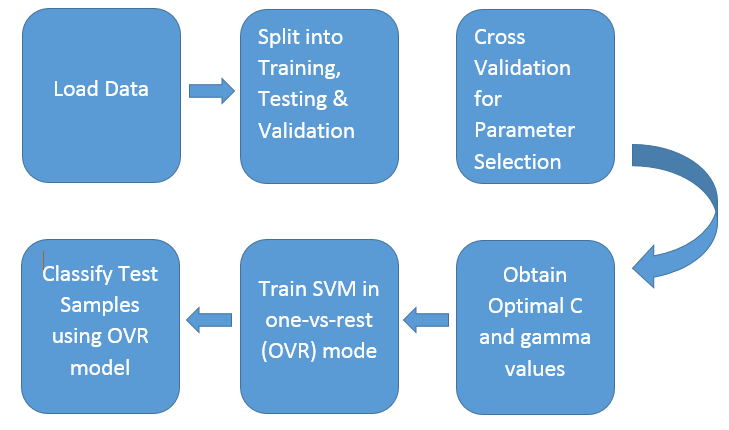
\includegraphics[scale=0.6] {fig_svmflow.png} 
 	   \caption{A typical classification model of SVM }
       \label{fig:svmflow}
\end{figure}
The gamma parameter defines how far the influence of a single training example reaches, with low values meaning `far` and high values meaning `close`. The C parameter trades off misclassification of training examples against simplicity of the decision surface. A low C makes the decision surface smooth, while a high C aims at classifying all training examples correctly. 
These parameters had to be fine-tuned to get the optimal values for classification. This was done using cross-validation and will be explained in the subsequent section. 

\subsection{Neural Networks}
\noindent
Artificial neural networks are the function approximators inspired by the biological process. If the system is dependent on the multiple parameters that are unknown, NN can be used to obtain the hidden parameters responsible for the known output.
\begin{figure}[!hbtp]
 	  \centering
 	   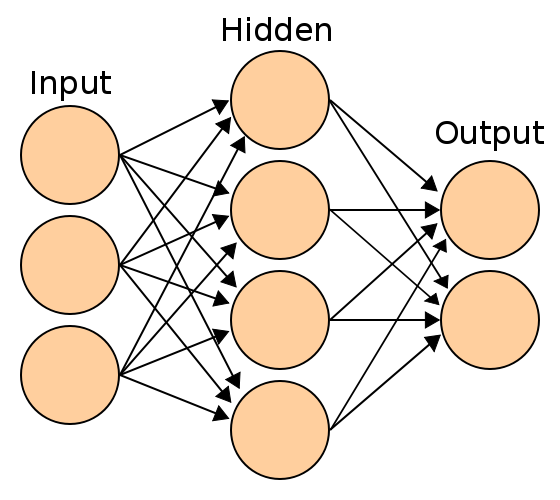
\includegraphics[scale=0.4] {fig_NN.png} 
 	   \caption{A typical NN model (source: Wikipedia) }
       \label{figNNtypical}
\end{figure}
\cref{figNNtypical} shows a typical NN model. First layer is the input layer which depends on the size of the data. Last layer is called as the output layer. Generally for a classification problem, outputs are binary numbers at a given class position. Hidden layers/intermediate layers are used for the large complex datasets with high dimensional unknowns.

In this project, a linear searching of optimal number of hidden layers and the number of neurons is performed. The weights are initialized with the random entries. Similarly, biases also follow the same argument.

\subsection{Error Analysis}
Many theoretical and experimental studies have shown the influence the capacity of a learning machine has on it`s generalization ability. Small capacity learning machines might not need huge training sets to achieve the best result. High capacity machines though might need large amounts of data to reach acceptable performance. The behavior of the difference between the training and test error as a function of the training set size is characterized by a measure quantifying the machine`s capacity. This measure is called the \enquote*{VC dimension} after Vladimir Vapnik and Alexey Chervonenkis. The VC dimension is an effective metric to measure the capacity of a learning machine for binary classification problems. For multiclass classification though, other concepts such as fat-shattering dimension, Natarajan dimension, Covering numbers and Rademacher complexity have been introduced. Due to constraints, the entire theory isn`t explained. Rather, important results and expressions have been mentioned (\cite{vapnik1971uniform}; \cite{haussler1995generalization}; \cite{tewari13learning}; \cite{abu2012learning}; \cite{murphy2012machine}).


In order to measure the predictive performance of a function $f : X \rightarrow Y$, we use a loss function. A loss function $l : Y \times Y \rightarrow R+$ is a non-negative function that quantifies how bad the prediction $f(x)$ is if the true label is $y$. In the classification case, binary or otherwise, a natural loss function is the 0-1 loss. Given a loss function, we can define the risk of a function $f : X \rightarrow Y$ as its expected loss under the true underlying distribution: $\mathsf{R}^N (f)$. Note that the risk of any function f is not directly accessible to the learner who only sees the samples. But the samples can be used to calculate the empirical risk of $f: R(f)$. Minimizing the empirical risk over a fixed class $F \subset YX$ of functions leads to a very important learning rule, namely empirical risk minimization (ERM). The excess risk of ERM relative to $fF$ can be decomposed as:
\begin{equation} \label{eq:raviEq1}
R(\hat{f_n}) - R(f^* \mathscr{F}) = (R(\hat{f_n}) - \hat{R}(\hat{f_n})) + (\hat{R}(\hat{f_n}) - \hat{R}(\hat{f*}\mathscr{F})) + (\hat{R}(f^* \mathscr{F})) + (\hat{R}(f^* \mathscr{F}) - R(f^* \mathscr{F}))
\end{equation}
Covering Numbers : Balls of radius $\alpha$ placed at elements of T cover the set T entirely. The covering number (at scale $\alpha$) of T is defined as the size of the smallest cover of T (at scale $\alpha$).
Structural Risk Minimization: Consider the classification setting with 0-1 loss (\cref{eq:raviEq2}). 
\begin{equation} \label{eq:raviEq2}
\displaystyle \E [R(\hat{f_n})] - R(f^*) \leq \min_{k} \left\lbrace\displaystyle \E[pen(k)] + (R(f^*_{\mathscr{F^{(b)}}}))\right\rbrace + \sqrt{\frac{log(ce)}{2m}}
\end{equation}
\cref{eq:raviEq3} Data Driven Penalties Using Rademacher Averages:
We can use the data dependent penalty to get the bound:
\begin{equation} \label{eq:raviEq3}
\displaystyle \E [R(\hat{f_n})] - R(f^*) \leq \min_{k} \left\lbrace 2 \mathscr{R}_n (\mathscr{F}^{(k)}) + (R(f^*_{\mathscr{F}^{(b)}}) - R(f^*))  * \sqrt{\frac{log k}{Cn}}\right\rbrace \sqrt{\frac{log (ce)}{2Cn}}
\end{equation}

\subsubsection*{Interpretation for SVM} 
The Radial Basis Function kernel that has been used for the model is capable of mapping onto the entire feature space. The dimension of it`s feature space is therefore infinite. For static learning, we have the following theorem, \enquote*{If a concept class C has infinite VC dimension, then C is not learnable by any static learning algorithm}. This isn`t the case for multiclass learning, where we make use of other notions like the \enquote*{effective VC-dimension} and \enquote*{covering numbers} which do not necessarily impose such hard constraints. For SVM, the original VC dimension doesn`t work well. Vapnik noticed that the VC-dimension of a SVM is 	h = dim (F) + 1.				
SVMs generally have very high VC dimensions. So, the value of the VC bound of the risk is also very high, possibly infinite Despite having an infinite error bound, the actual performance of the SVM is pretty good. Though the SVM is distribution free, for a given training task, the distribution is already known. Hence, the SVM might not reach it`s full capacity while training. It was for this reason that Vapnik introduced the concept of effective VC dimension, which is a measurement of the capacity of not only the SVM, but also the sample complexity. 


\section{Methodology} \label{sec:methodology}
\noindent
This section provides a brief overview of the entire procedure, beginning right from hypothesis and class label selection, all the way to performance measures and error analysis. 

In \cref{fig:methodology} a flowchart is provided to visualize the framework. Each stage in this flowchart represents a class (or) group of operations. These classes incorporate the several intermediate steps in the procedure. An explanation of each step is provided after the flowchart. 
\begin{figure}[!hbtp]
 	  \centering
 	   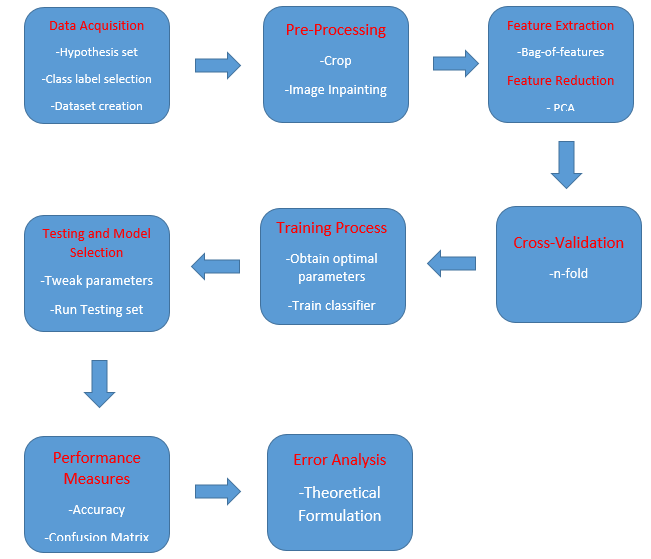
\includegraphics[scale=0.9] {fig_methodology.png} 
 	   \caption{Various phases for the project}
       \label{fig:methodology}
\end{figure}


The list of the methods used in this work are enumerated as below:
\begin{enumerate}
\subsection*{Model}
  \item Hypothesis set: In this work, hypothesis sets includes all the space consists of the SVM and NN models.
  
  \item Class labels selection: Given, dataset totally consists of 16 to 17 classes. Out of which, nine classes are selected based on the importance of the classes and available computational resources.
  
  \item Dataset:  Dataset is obtained from converting 100 sewer pipeline videos to images. Images are manually labeled and outliers are filtered. Subsequently, training, validation and testing datasets are randomly selected.
  
  \subsection*{Pre-processing}
  \item Crop: All the images are overlaid with text. This extra text and just behaves as noise in the image. Owing to the low quality of the image and the relatively huge size of the mask, inpainting algorithms too failed to provide us with a reasonable approximation. Thus, we adopted the option of cropping the images so that the part overlaid with text is cut and is no longer considered. 
  
  \item Inpaint: The patches at the bottom of the image which display the date, time and location are comparatively smaller than those at the top of the image. Thus, it was possible to apply the inpainting algorithm on them. This algorithm, which is based on a weighted minimum norm-based implementation will be discussed in the forthcoming section.
  
  \item Feature Extraction: In order to automatically extract the features from the given images bag-of-features \citep{csurka2004visual} is used obtain a very high dimenisonal feature vectors.
  
  \item Split into training, testing and validation: Dataset is been divided into three subsets which has a ration 0.6:0.1:0.3, training, validation and testing respectively.
  
  \item Feature Reduction : Since the feature matrix obtained for each of the sets is huge, it justifies considering some sort of feature reduction method to reduce the dimensionality of the data. The method we`ve used is Principal Component Analysis (PCA) and it`ll be summarized shortly.
  
\subsection*{Training Process}
\item Cross validation: Cross validation is a model validation technique for assessing how the results of a statistical analysis will generalize to an independent data set.

\item Obtain optimal parameters: The cross validation step gives us the optimal value/s of the parameter/s needed for the model. These could be the penalty term (C) or gamma in case of SVMs or could be the number of hidden layers, number of nodes, etc. 

\item Train Classifier: Once the optimal parameters are obtained, the classifier can be trained.

\subsection*{Testing, Validation and model Selection}
\item Test on validation set: Once a model is created after learning the training data, the model is tested on the validation set. Even though we carried out This could be due to a local minima. The parameters of the model can be tweaked if the results of the validation aren’t satisfactory. These trial are repeated till we are satisfied with the model.

\item Obtain robust model: The continuous improvement of the model by repetitive trials of the validation data ensures that the final model we obtain is very robust and resilient to overfitting.

\item Test on testing set: The model is then tested on the testing set.

\item Performance measures: Several performance measures such as accuracy, misclassification rate, confusion matrix, etc are used to judge the performance of the classifier on the testing data. 

\subsection*{Error Analysis}
\item Error measure: Finally, check whether the out-of-sample error satisfies the expression provided for the error bound.
 
\end{enumerate}

\section{Implementation} \label{sec:implementation}
\subsection{Feature Space}
\noindent
Images of the sewer pipeline are extremely diverse and challenging as shown in \cref{fig:pipeImages}. In this figure different class images are shown. As in the image it is evident how diverse the images are in colorspace and also in shape characteristics.
\begin{figure}[!hbtp]
 	  \centering
 	   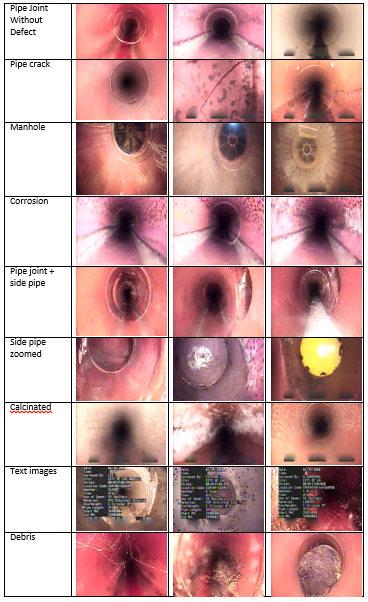
\includegraphics[scale=1.3] {fig_pipeImgs.png} 
 	   \caption{Various classes of images}
       \label{fig:pipeImages}
\end{figure}
In this work, a histogram of a quantized vector is considered to represent repetitions of the image patches (explained in feature extraction section). 


\subsection{Pre-processing and Feature Extraction}
Once the class labels were decided, then began the pre-processing part. Each image underwent the following stages of pre-processing and feature extraction:

\subsubsection*{Cropping the image}
All the images are overlaid with text. This extra text and just behaves as noise in the image. Owing to the low quality of the image and the relatively huge size of the mask, inpainting algorithms too failed to provide us with a reasonable approximation. Thus, we adopted the option of cropping the images so that the part overlaid with text is cut and is no longer considered. 

\subsubsection*{Image inpainting}
Inpainting is the process of reconstructing lost or deteriorated parts of images and videos. The notion of digital inpainting was firstintroduced in the paper by \cite{bertalmio2000image}. Smart digital inpainting models, techniques, and algorithms have broad applications in image interpolation, photo restoration, zooming and super-resolution, primal-sketch based perceptual image compression and coding, and the error concealment of (wireless) image transmission, etc. 
Inpainting is rooted in the restoration of images. The methodology followed is : 
\begin{itemize}
\item The global picture determines how to fill in the gap. The purpose of inpainting is to restore the unity of the work.
\item	The structure of the gap surroundings is supposed to be continued into the gap. Contour lines that arrive at the gap boundary are prolonged into the gap.
\item The different regions inside a gap, as defined by the contour lines, are filled with colors matching for those of its boundary.
\item The small details are painted, i.e. \enquote{texture} is added.
\end{itemize}


\paragraph{Inpainting problem:} 
Given an image and a region $\Omega$ inside it, the inpainting problem consists in modifying the image values of the pixels in $\Omega$ so that this region does not stand out with respect to its surroundings.

Our Method : Our method of image inpainting was based off a weighted minimum norm implementation. Given the image, we generate a mask of the image indictating the locations at which text is present. The algorithm makes use of the mask to determine the region in which inpainting is to be done. Once this region has been identified, all the pixels from this region are made zero. This can be considered equivalent to removing that region from the image. The missing pixels have to be replaced with values in such a way that the $\mathsf{L2}$-norm of the solution is the least. The image (solution) is multiplied with a weighting matrix and at every iteration, the goal is to choose an x that minimizes the l2-norm of the solution. Different constraints are then applied to the image. For example, the image does not have continuous 2D edges, but instead has\enquote{jagged} edges in locations where the text occluded an image edge. This type of information could have been restored if we had used a 2D version of the $WMN$ constrain that imposed both horizontal and vertical smoothness. Alternatively, we could have used the prior information that this type of painting should have a fairly consistent spatial texture, or the constraint that the painting should be compressible in a wavelet transform, or the constraint that the painting is possibly compressible under a low-rank matrix representation of the image. 
\begin{equation}
\hat{X}_{WMN} = (T^H T)^{-1} A^H (A(T^H T)^{-1})A^H)^{-1}b
\end{equation}
Here, $\hat{X}_{WMN}$ is the final solution we are interested in. 
\begin{figure}[!hbtp]
 	  \centering
 	   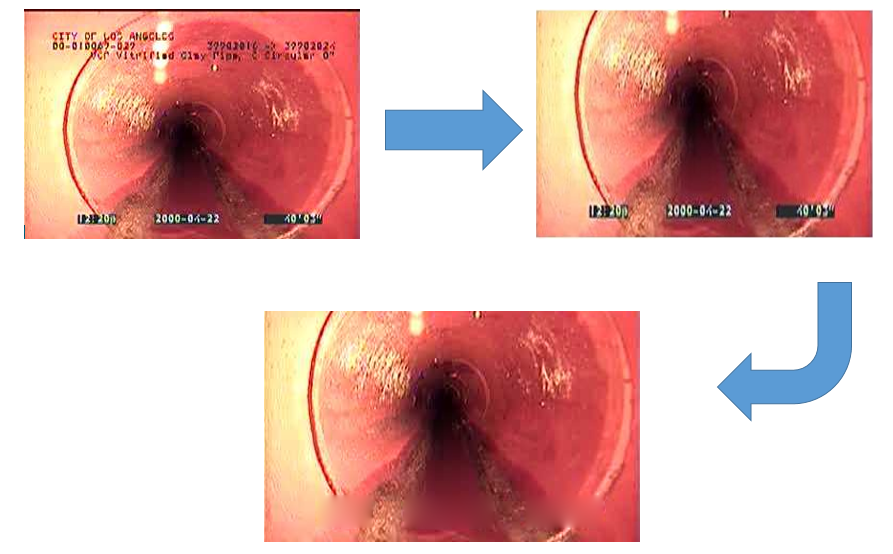
\includegraphics[scale=0.5] {fig_inpaint.png} 
 	   \caption{An inpainted image}
       \label{fig:inpaint}
\end{figure}


\subsubsection*{Feature extraction}
In this work, automatic feature extraction such as bag-of-features is been used to extract the feature vector from the given image samples. Firstly, image descriptors such as Speeded Up Robust Features (SURF) is used to obtain the key-points in images (refer \cref{fig:surfPoints}). Secondly, descriptor vector that contains the visual information around the key-point is formed for each images. 
\begin{figure}[!hbtp]
 	  \centering
 	   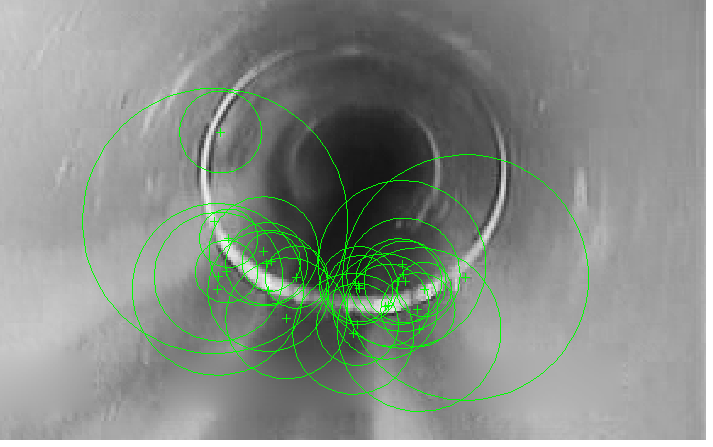
\includegraphics[scale=0.5] {surf.png} 
 	   \caption{A SURF detector points}
       \label{fig:surfPoints}
\end{figure}
Thirdly, key-point descriptor are obtained for all the images in the dataset. Fourthly, these feature descriptors are clustered to produce a visual vocabulary of $k$ words. Fifthly, in each image the count of the visual words are considered and an histogram is obtained. This vector dimension is equal to the dimension of the feature vector. Lastly, each vector is normalized to a unit vector and to have a consistency. For more details please refer to \cite{csurka2004visual}.

\subsubsection*{Feature reduction}
Since the feature matrix obtained for each of the sets is huge, it justifies considering some sort of feature reduction method to reduce the dimensionality of the data. The method we`ve used is Principal Component Analysis (PCA). Principal component analysis (PCA) is a statistical procedure that uses an orthogonal transformation to convert a set of observations of possibly correlated variables into a set of values of linearly uncorrelated variables called principal components. PCA was invented in 1901 by Karl Pearson \citep{jolliffe2005principal}. The number of principal components is less than or equal to the number of original variables. This transformation is defined in such a way that the first principal component has the largest possible variance (that is, accounts for as much of the variability in the data as possible), and each succeeding component in turn has the highest variance possible under the constraint that it is orthogonal to (i.e., uncorrelated with) the preceding components. The principal components are orthogonal because they are the eigenvectors of the covariance matrix, which is symmetric. The principal components as a whole form an orthogonal basis for the space of the data. The first principal component is a single axis in space. When you project each observation on that axis, the resulting values form a new variable. And the variance of this variable is the maximum among all possible choices of the first axis. The second principal component is another axis in space, perpendicular to the first. Projecting the observations on this axis generates another new variable. The variance of this variable is the maximum among all possible choices of this second axis.
The choice of how many dimensions to reduce to is made through visual inspection of the plot of the eigenvalues, also called the `scree-plot`. The plot for our feature dimension is provided below.
\begin{figure}[!hbtp]
 	  \centering
 	   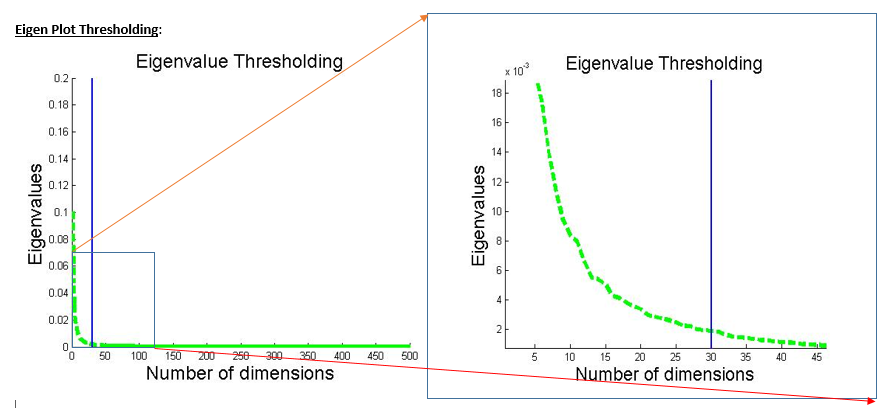
\includegraphics[scale=0.65] {fig_eigValPlot.png} 
 	   \caption{A scree plot of the PCA latency (Eigen values)}
       \label{fig:pcaScreePlot}
\end{figure}
From the \cref{fig:pcaScreePlot}, original number of dimensions, D = 500 and reduced number of dimensions, D' = 30.

\subsection{Training Process}
Once filtered and processed feature matrix is ready, we can begin the training process. The first step is Cross Validation. Cross-validation, sometimes called rotation estimation, is a model validation technique for assessing how the results of a statistical analysis will generalize to an independent data set. The goal of cross validation is to define a dataset to \enquote{test} the model in the training phase (i.e., the validation dataset), in order to limit problems like overfitting, give an insight on how the model will generalize to an independent data set (i.e., an unknown dataset, for instance from a real problem), etc. One round of cross validation involves. 

Partitioning a sample of data into complementary subsets, performing the analysis on one subset (called the training set), and validating the analysis on the other subset (called the validation set or testing set). To reduce variability, multiple rounds of cross-validation are performed using different partitions, and the validation results are averaged over the rounds.

Cross-validation is important in guarding against testing hypotheses suggested by the data (called type III errors) especially where further samples are hazardous, costly or impossible to collect.

\begin{enumerate}
\item Obtain optimal parameters: The cross validation step gives us the optimal value/s of the parameter/s needed for the model. These could be the penalty term (C) or gamma in case of SVMs or could be the number of hidden layers, number of nodes, etc. 

The optimal parameters obtained for the SVM with RBF Kernel are :  C = 2 and $\gamma$ = 16.

\item Train Classifier in OVR (one-vs-rest mode): Once the optimal parameters are obtained, the classifier can be trained.
In machine learning, multiclass or multinomial classification is the problem of classifying instances into more than two classes. While some classification algorithms naturally permit the use of more than two classes, others are by nature binary algorithms; these can, however, be turned into multinomial classifiers by a variety of strategies.
\end{enumerate}

\subsubsection*{One-vs.-rest}
The one-vs.-rest (or one-vs.-all, OvA or OvR) strategy involves training a single classifier per class, with the samples of that class as positive samples and all other samples as negatives. This strategy requires the base classifiers to produce a real-valued confidence score for its decision, rather than just a class label; discrete class labels alone can lead to ambiguities, where multiple classes are predicted for a single sample. 

\subsubsection*{One-vs.-one}
In the one-vs.-one (OvO) reduction, one trains K (K - 1) / 2 binary classifiers for a K-way multiclass problem; each receives the samples of a pair of classes from the original training set, and must learn to distinguish these two classes. At prediction time, a voting scheme is applied: all K (K - 1) / 2 classifiers are applied to an unseen sample and the class that got the highest number of "+1" predictions gets predicted by the combined classifier. Like OvR, OvO suffers from ambiguities in that some regions of its input space may receive the same number of votes.
\begin{center}
Number of training samples = 8,617 \\
Original Dimension (D)     = 500 \\
New Dimension (D') 	       = 30.
\end{center}
The model is tested repeatedly on the validation set until suitable parameters are obtained. This reduces the extent of overfitting or underfitting. 


\subsection{Testing, Validation and Model Selection}
\begin{enumerate}
\item Test on validation set: Once a model is created after learning the training data, the model is tested on the validation set. Even though we carried out This could be due to a local minima. The parameters of the model can be tweaked if the results of the validation aren’t satisfactory. These trial are repeated till we are satisfied with the model.

\item Obtain robust model: The continuous improvement of the model by repetitive trials of the validation data ensures that the final model we obtain is very robust and resilient to overfitting.

\item Test on Testing Set: The model is then tested on the testing set.

\item Performance Measures: Several performance measures such as accuracy, misclassification rate, confusion matrix, etc are used to judge the performance of the classifier on the testing data. 
\begin{figure}[!hbtp]
 	  \centering
 	    \subfloat[Decision boundary for testing set]{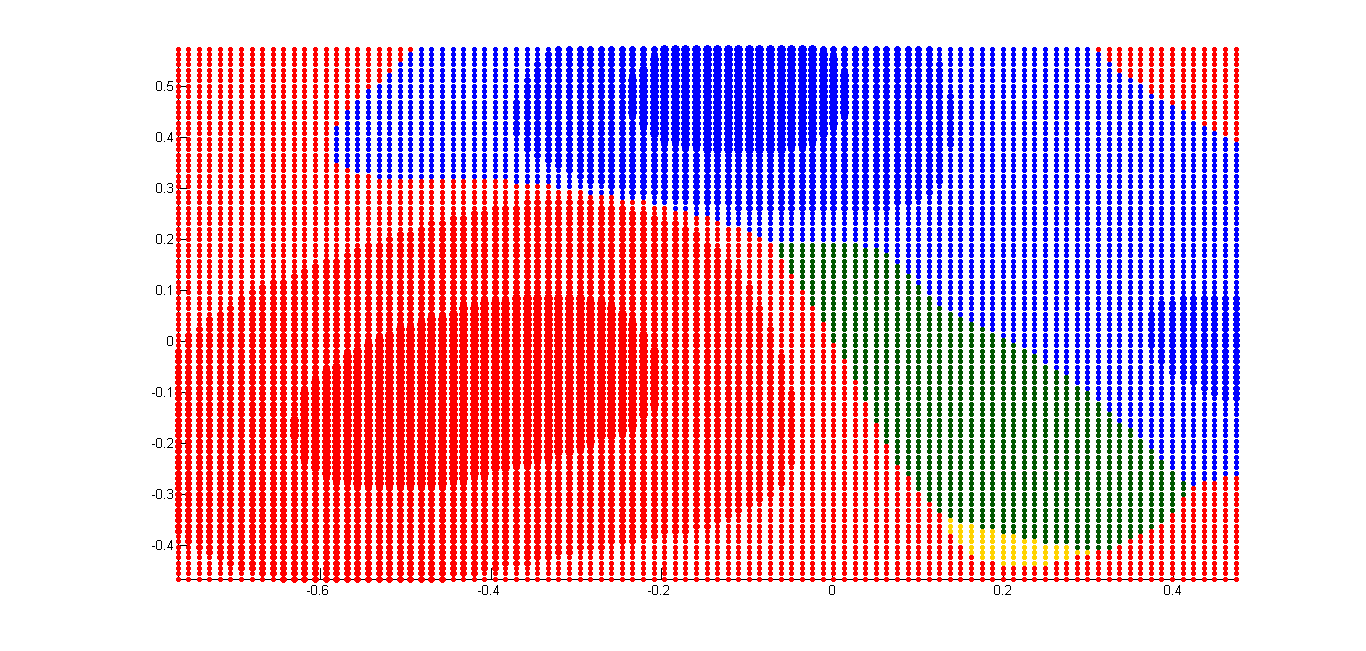
\includegraphics[scale=0.3] {svm_dec_bndry.png} \label{fig:svmbndry}}
  		\quad
  		\subfloat[Data points scatter plot]{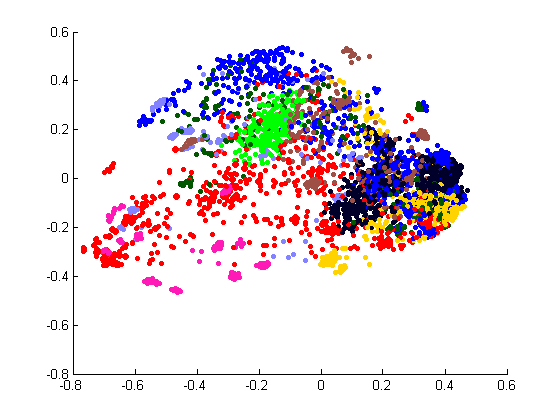
\includegraphics[scale=0.3] {svm_scatter.png} \label{fig:svmscatter}}
 	   \caption{Decision boundary of a SVM classifier }
       \label{fig:deci_bndry}
\end{figure}

\end{enumerate}

\section{Final Results} \label{sec:final_results}
\noindent
A new labeled dataset of a magnitude 14362 images is created for this project. This dataset consists of nine different classes. Namely: 1. Pipe joint without defect, 2. debris, 3. corrosion, 4. calcinated, 5. text images,  6. pipe crack, 7. pipe joint + side pipe, 8. side piped zoomed, and 9. manholes. The distribution of these classes is shown in \cref{fig:class_distribution}.
\begin{figure}[!hbtp]
 	  \centering
 	   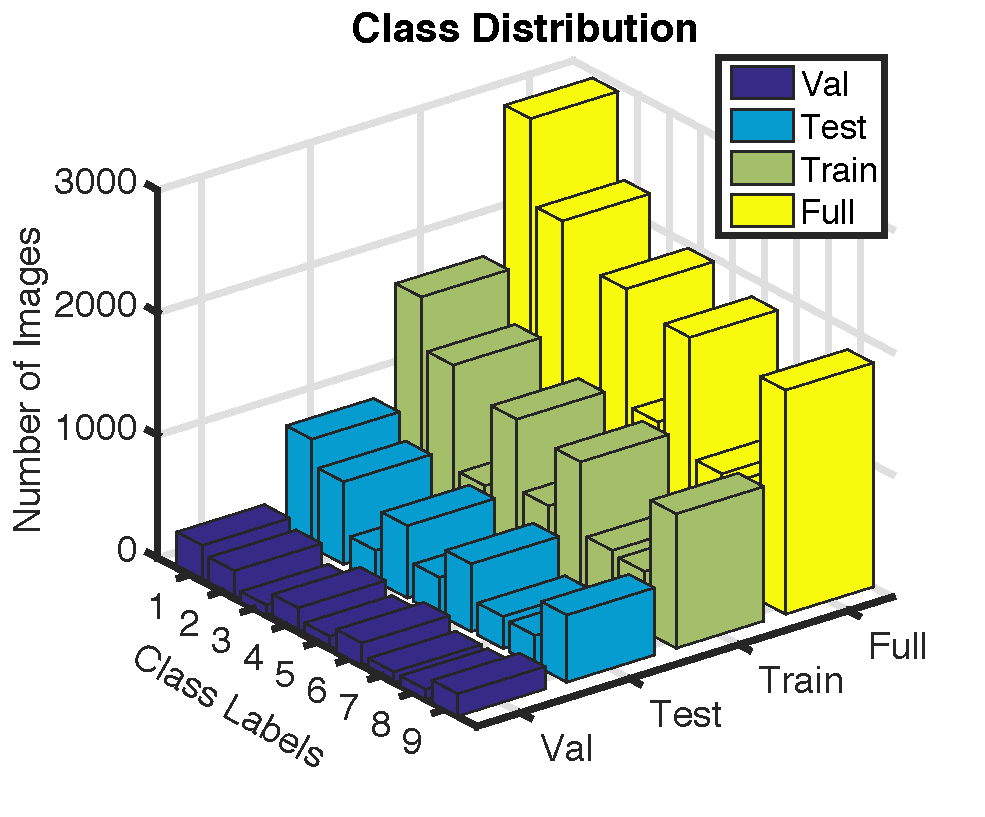
\includegraphics[scale=0.75] {fig_class_distribution.pdf} 
 	   \caption{Distribution of the Dataset }
       \label{fig:class_distribution}
\end{figure}

The dataset is randomly shuffled and divided into three subsets like: training, testing and validation (60, 30 and 10 \%) respectively. Each of these sets are separately encoded in order to produce the feature matrices. Special care is taken such that their labels are still preserved while shuffling.

In this work, two non-linear classifiers are used to perform the object classification. The results of our method are shown in the below sections.
\subsection{SVM}
We made use of an RBF kernel in order to implement the multiclass classification using SVMs. The parameters affecting the performance of the RBF kernel are: C (penalty parameter) and gamma. 
These parameters were selected on the basis of the performance of the model on the validation set.
We performed 3-fold cross validation. The default values used by LIBSVM are:
C = 1 , gamma = 1/(number of features)
The values we obtained after k = 3 fold cross validation are:
C = 2 , gamma = 16.

\begin{table}[!htbp]
\centering
 \begin{tabular}{ l c c }
 \hline
 Class Label & Validation Accuracy (\%) &  Testing Accuracy (\%)  \\ [0.5ex]
 \hline\hline \\ [-1.5ex]
	Pipe Joint Without Defect & 79.2768 & 77.4553  \\ 
	Pipe Crack & 84.5619 & 85.1405  \\ 
	Pipe Joint + Side pipe  & 94.2281 & 94.1723  \\ [1ex]
	Side pipe zoomed  & 86.3004 & 86.1853  \\ [1ex]
	Manhole  & 92.9068 & 92.9185  \\ [1ex]
 	Debris  & 87.1349 & 87.1604  \\ [1ex]
	Corrosion  & 93.9499 & 93.9401  \\ [1ex]
	Calcinated  & 94.2976 & 94.3348  \\ [1ex]
	Text Images  & 87.274 & 87.2765  \\ [1ex]
\hline \\ [-1.5ex]
	Mean accuracy  & 88.88 & 87.73  \\ [1ex]
 \hline
 \end{tabular}
  	   \caption{Classifier performance for SVM}
       \label{tab:classifier_performance_svm}
\end{table}

\cref{fig:obssvm} shows the observation made on validation sets. The figure on the left displays the decision values on the validation set. For a given class k, the greenish-blue values denote the samples belonging to the same class k and values that are brighter, towards the red spectrum belong to other classes. These indicate the misclassified samples.The figure on the right provides us with the output labels for class k. Since SVMs use the one-vs-rest methodology, each class is compared to the rest as a whole and labels are set. Similar to the previous figure, the red values indicate that the output labels of those samples are different from the labels assigned to samples belonging to class k. 
\begin{figure}[!hbtp]
 	  \centering
 	   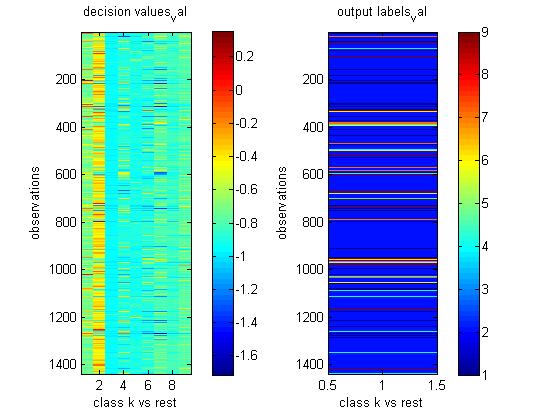
\includegraphics[scale=0.75] {svm_dec_val.png} 
 	   \caption{Observations SVM}
       \label{fig:obssvm}
\end{figure}


\subsection{Neural network}
In this  work, multi-layer neural networks are considered to learn the data and to predict the test class labels. \cref{fig:errorNNHLS} shows the
\begin{figure}[!htb]
  \centering
  \subfloat[One hidden layer]{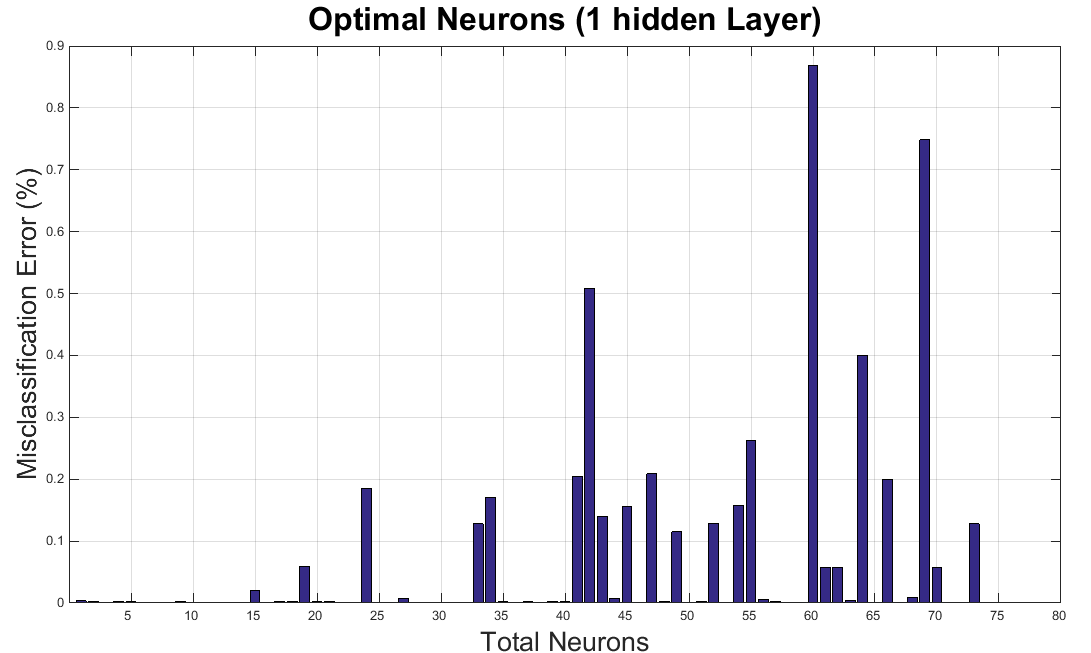
\includegraphics[scale=0.4] {fig_optiNeuron_1HL.png} \label{fig:1HL}}
  \\
  \subfloat[Two hidden layer]{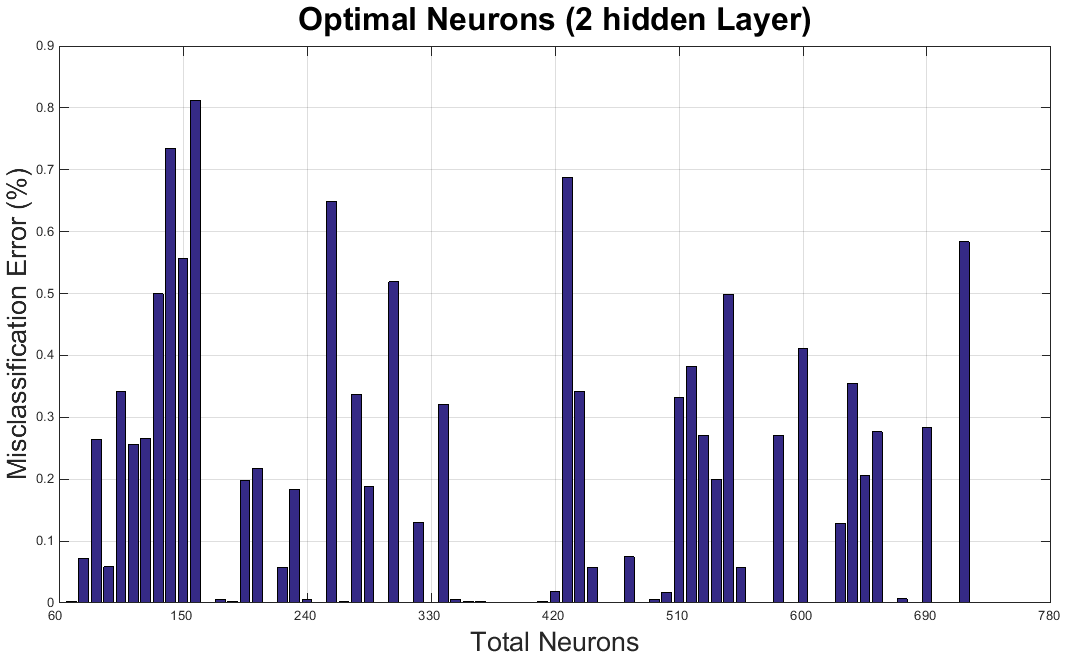
\includegraphics[scale=0.4] {fig_optiNeuron_2HL.png} \label{fig:2HL}}
  \\   
  \subfloat[Three hidden layer]{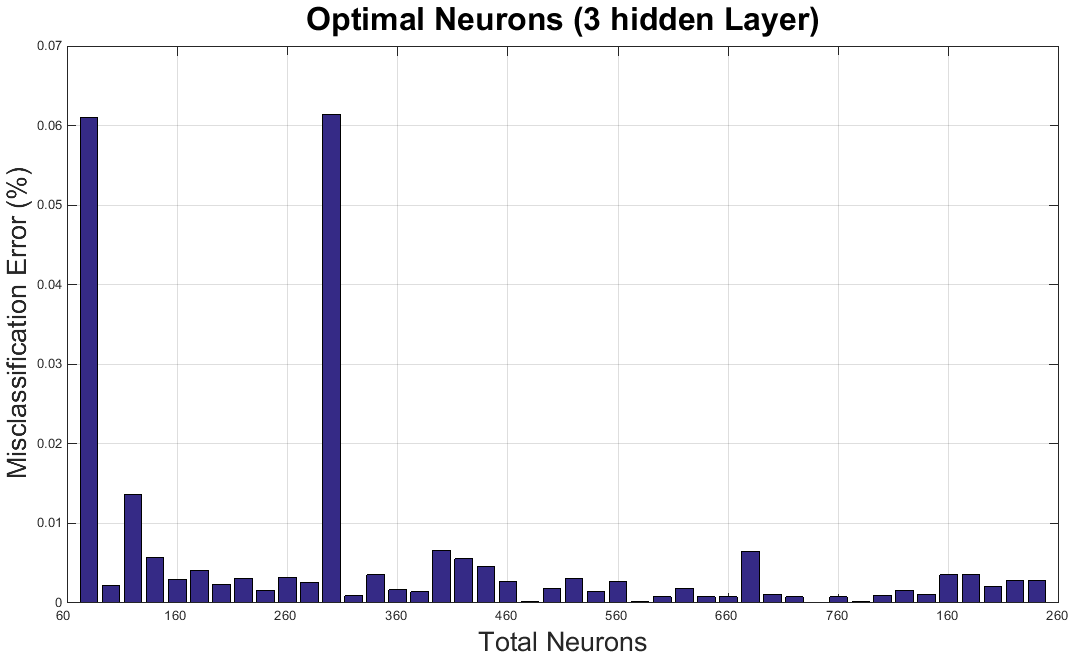
\includegraphics[scale=0.4] {fig_optiNeuron_3HL.png} \label{fig:3HL}}
  \caption{Misclassification error for NN with 1-2-3 hidden layers and various neurons}
  \label{fig:errorNNHLS}
\end{figure}
misclassification error rate of neural network with one, two and three hidden layers. Execution time was more than 15 hours to train, validate and test all the dataset for various number of neuron units. It is noted that the best test set misclasfficiation rate are: one hidden layer with 65 neurons gave 6.96282e-05, two layers with [570,210] neurons provided 0 and 6.9628e-05 for [420,120,20] neuron units (refer \cref{tab:classifier_performance_ffnn}).

\begin{table}[!htbp]
\centering
 \begin{tabular}{ l l  c c }
 \hline
 Classifer type & Number of Neurons & Best Val. Accuracy (\%) &  Best Testing Accuracy (\%)  \\ [0.5ex]
 \hline\hline \\ [-1.5ex]
	NN 1 HL & 65 & 97.2768 & 99.99  \\ 
	NN 2 HL & 570, 210 &  95.6712 & 100   \\ 
	NN 3 HL & 420, 120, 20 & 96.5619 & 99.99  \\ 
\hline \\ 
 \hline
 \end{tabular}
  	   \caption{Classifier performance for FFNN}
       \label{tab:classifier_performance_ffnn}
\end{table}

\section{Interpretation} \label{sec:interp} %\enquote{igboibi}
\noindent
As can be observed from the results above, Neural Networks perform extremely well on the given data. They are capable of accurately classifying the images into one amongst 9 classes. SVM though, doesn`t enjoy this performance. It gives slightly poorer performance than NN does. A possible reason could be the use of Radial Basis Function (RBF) as a kernel instead of a linear kernel. Additionally, multiclass SVMs follow the principle of one-vs-rest (OVR). Thus, even though the individual classification results are good, the overall performance could be quite poor. In OVR, the `rest` is huge and can get separated easily from the main class. Combining all the single classifications could lead to some competitive effect between winners. This could be the reason behind the low accuracy.

In neural network model, \cref{fig:errorNNHLS} it was noted that increasing the number of neuron units overfit the data and worked poorly for testing data for one hidden layer NN. In contrast, three hidden layer system performed well for increase in the neurons. But, two layer system on an average under performed. Three layer network for lower neurons worked poorly, as the non-linearity increased with number of layers. Even, one hidden layer with five neurons is able to provide a classifier that has the misclassification error rate of 0.003411. Thus, it is evident that an optimal number of neurons with one layer is sufficient for good classification rate. On the other hand, neural network with two or three hidden layers (permutations of neurons) is computationally heavy.

It is worthwhile to note, that both SVM and FFNN worked well on an average owing to the fact that the overfiting is relaxed due to the large number of training samples 8617. For validation and testing, 1438 and 4307 images are used respectively. As part of a separate experiment, the training set size was decreased, keeping the validation and testing set sizes the same. It was observed that the accuracy drastically decreased in this case, decreasing by almost 50\%, which was to be expected.


%%%%%%%%%%%%%%%%%%%%%%%%%%%%%%%%%%%%%%%%%%%%%%%%%%%%%%%%%%%%%%%%%%%%%%%%%%%%%%%%%%%%%%%%%%%%%%%%%%%%%%%%%%%%%%%%%%%%%%%%%%%%%%%
\section{Summary, Conclusions and Future Work} \label{sec:summary_conclusion}
\noindent
In this work, sewer pipeline defect and non-defect image classification is considered. A new dataset has been manually labeled and partitioned into training, testing and validation sets. A total of 14362 images under nine classes are formed by using 100 randomly selected sewer pipe videos. Furthermore, two non-linear classifiers such as SVM and FFNN are used to predict the class labels. These classifiers are selected based on the number of samples and prior observations made in the research community. Lastly, an attempt has been made to understand the generalization bound for multiple classes as an extension to the coursework.    

Results obtained from both the classifiers were surprising and satisfactory. It is observed that non-uniform distribution of the images in each class might have biased the accuracy of the SVM classifier. This is due to the fact that current classification method is one-vs.-rest. Neural network even with one layer and five neurons performed tremendously well with a classification accuracy more than 99.5\%. Lastly,higher training samples relaxed the overfitting and helped in the good performance of the classifiers.  

As a continuation, in the near future some of these suggestions will be implemented. Firstly, instead of using image inpainting, a video algorithm will be used to remove the text autonomously. Secondly, each images are obtained by frame-extraction of a video. Thus, augmenting temporal scale might be an interesting problem to solve. Thirdly, due to time constraints, an hybrid parallel algorithm will be developed. Fourthly, bag-of-feature, although performed very well, it is worth to consider the explicit shape characteristics to localize the objects of interest (includes intra-class items too) within each image. Lastly, a closed form solution of generalization bound that is pertinent for SVM and FFNN will be improved.

%%%%%%%%%%%%%%%%%%%%%%%%%%%%%%%%%%%%%%%%%%%%%%%%%%%%%%%%%%%%%%%%%%%%%%%%%%%%%%%%%%%%%%%%%%%%%%%%%%%%%%%%%%%%%%%%%%%%%%%%%%%%%%%
\section{Acknowledgments} 
\noindent
Firstly, the authors are highly thankful to Professor Keith Jenkins for his teaching and guiding throughout the semester. Secondly, the authors would also like to thank Shuyang Sheng, TA for EE 660 for his immense support in explaining homework assignments and project guidelines. Lastly, the authors are thankful to graduate students Vinay Hegde and Tanmay Patil working in USC, SHM lab for their conscientious efforts in creating the world's largest sewer pipeline ground-truth image database!

\clearpage	
%\nocite{*}

% Bibtex
\bibliographystyle{chicago}
\bibliography{Report-SewerPipe}

\clearpage
%\renewcommand*\appendixpagename{Appendix}
%\renewcommand*\appendixtocname{Appendix}
\begin{appendices}
\section{Main Code}
\lstinputlisting{C:/Users/Preetham/Desktop/Report/matlab/Main.m}
\lstinputlisting{C:/Users/Preetham/Desktop/Report/matlab/shravan_multisvm_t1.m}
\lstinputlisting{C:/Users/Preetham/Desktop/Report/matlab/NNClassifier.m}

\section{Sub-routines}
\lstinputlisting{C:/Users/Preetham/Desktop/Report/matlab/crop.m}
\lstinputlisting{C:/Users/Preetham/Desktop/Report/matlab/cropnMask.m}
\lstinputlisting{C:/Users/Preetham/Desktop/Report/matlab/filenamesort.m}
\lstinputlisting{C:/Users/Preetham/Desktop/Report/matlab/generate_Ai.m}
\lstinputlisting{C:/Users/Preetham/Desktop/Report/matlab/MainInputs.m}
\lstinputlisting{C:/Users/Preetham/Desktop/Report/matlab/largesScaleImInpaint.m}
\lstinputlisting{C:/Users/Preetham/Desktop/Report/matlab/inpaint.m}
\lstinputlisting{C:/Users/Preetham/Desktop/Report/matlab/makeLabelArray.m}
\lstinputlisting{C:/Users/Preetham/Desktop/Report/matlab/makePartitions.m}
\lstinputlisting{C:/Users/Preetham/Desktop/Report/matlab/plot3Dbargraph.m}
\lstinputlisting{C:/Users/Preetham/Desktop/Report/matlab/shufflerCallBacks.m}
\lstinputlisting{C:/Users/Preetham/Desktop/Report/matlab/shuffleNcopy.m}
\lstinputlisting{C:/Users/Preetham/Desktop/Report/matlab/shuffleFeatMatLabel.m}
\end{appendices}


% Biblatex
%\printbibliography [heading=bibintoc]
\end{document}